\documentclass[french]{article}
\usepackage{amssymb, amsmath, mathtools} %pour les mathématiques
\usepackage{fontspec}
\usepackage{xunicode}
\usepackage[a4paper]{geometry}
\usepackage{babel}
%\usepackage[xetex,hiresbb]{graphicx}
\usepackage{graphicx}
%\usepackage{sidecap}   % to place caption beside a figure
%\usepackage{wrapfig}   % wrapping text around figures
\usepackage{caption}   % to have subfigures within figures
\usepackage{subcaption}
\usepackage{float}
\floatstyle{boxed}
\restylefloat{figure}

% http://en.wikibooks.org/wiki/LaTeX/Floats,_Figures_and_Captions

\begin{document}


% les chemins ou sont stockées les images
%\graphicspath{ {~/f/CARTOGRAPHIE/Plans/2_Topo_EnCours/hotel_de_ville/20131210/Station\ 1/Points\ cible\ S1/} }
\graphicspath{{images/}{~/}{~/f/CARTOGRAPHIE/Plans/2_Topo_EnCours/hotel_de_ville/20131210/Station\ 1/Points\ cible\ S1/}}




\begin{titlepage}
  \begin{center}
    \vspace*{1cm}

    \Huge
    \textbf{Ville de La Rochelle}

    \vspace{0.5cm}
    \LARGE
    Hôtel de Ville

    \vspace{1.5cm}

    \textbf{Surveillance de la Façade Renaissance}

    \vfill

    Rapport N°1

    \vspace{0.8cm}

    %
\includegraphics[width=0.4\textwidth]{test.jpg}

    \Large
    Service Cartographie\\
    Direction Gestion Espace Public et Batiments\\
    Direction Générale des Services Techniques\\
    Ville de La Rochelle\\
    \date{-}

  \end{center}
\end{titlepage}

\thispagestyle{plain}
\begin{center}
  \Large
  \textbf{Surveillance de la Façade Renaissance\\de l'Hôtel de Ville}

  \vspace{0.4cm}
  \large
  Ville de La Rochelle

  \vspace{0.4cm}
  \textbf{Mesures du Service Cartographie}

  \vspace{0.9cm}
  \textbf{Résumé}
\end{center}

Le 4 décembre 2013, il a été constaté que la façade Renaissance semblait avoir subi, 
au droit de la seconde baie à droite, un mouvement de basculement vers l'intérieur.
Dans un rapport daté du 9 décembre 2013, Philippe Villeneuve, Architecte en Chef des 
Monuments Historiques, préconise de surveiller l'évolution de ce mouvement.

La surveillance de cette façade consiste à mesurer de manière périodique les distances 
entre des points fixes et des points cibles disposés sur cette façade.
L'évolution de ces distances est reportée dans ce rapport hebdomadaire.


\section{Les Points cibles}
Les points cibles
% debut d'une premiere figure
%\begin{figure}[!h]
%\centering
%
\includegraphics[width=\textwidth]{mydessin.pdf}
%\includegraphics[width=100pt]{~/f/CARTOGRAPHIE/Plans/2_Topo_EnCours/hotel_de_ville/20131210/Station\ 1/Points\ cible\ S1/P1020538.JPG}
%\includegraphics[width=100pt]{P1020538.JPG}
%\includegraphics[width=300pt,keepaspectratio=true,trim=0 0 300 300]{P1020538.JPG}
%\includegraphics[bb=0 0 2880 2160,trim=0 0 1000 1000,width=300pt,keepaspectratio=true]{P1020538.JPG}
%\includegraphics[trim=0 0 1000 1000,width=300pt,keepaspectratio=true]{P1020538.JPG}
%\includegraphics[bb=0 0 2880 2160,width=18cm,keepaspectratio=true]{P1020538.JPG}
%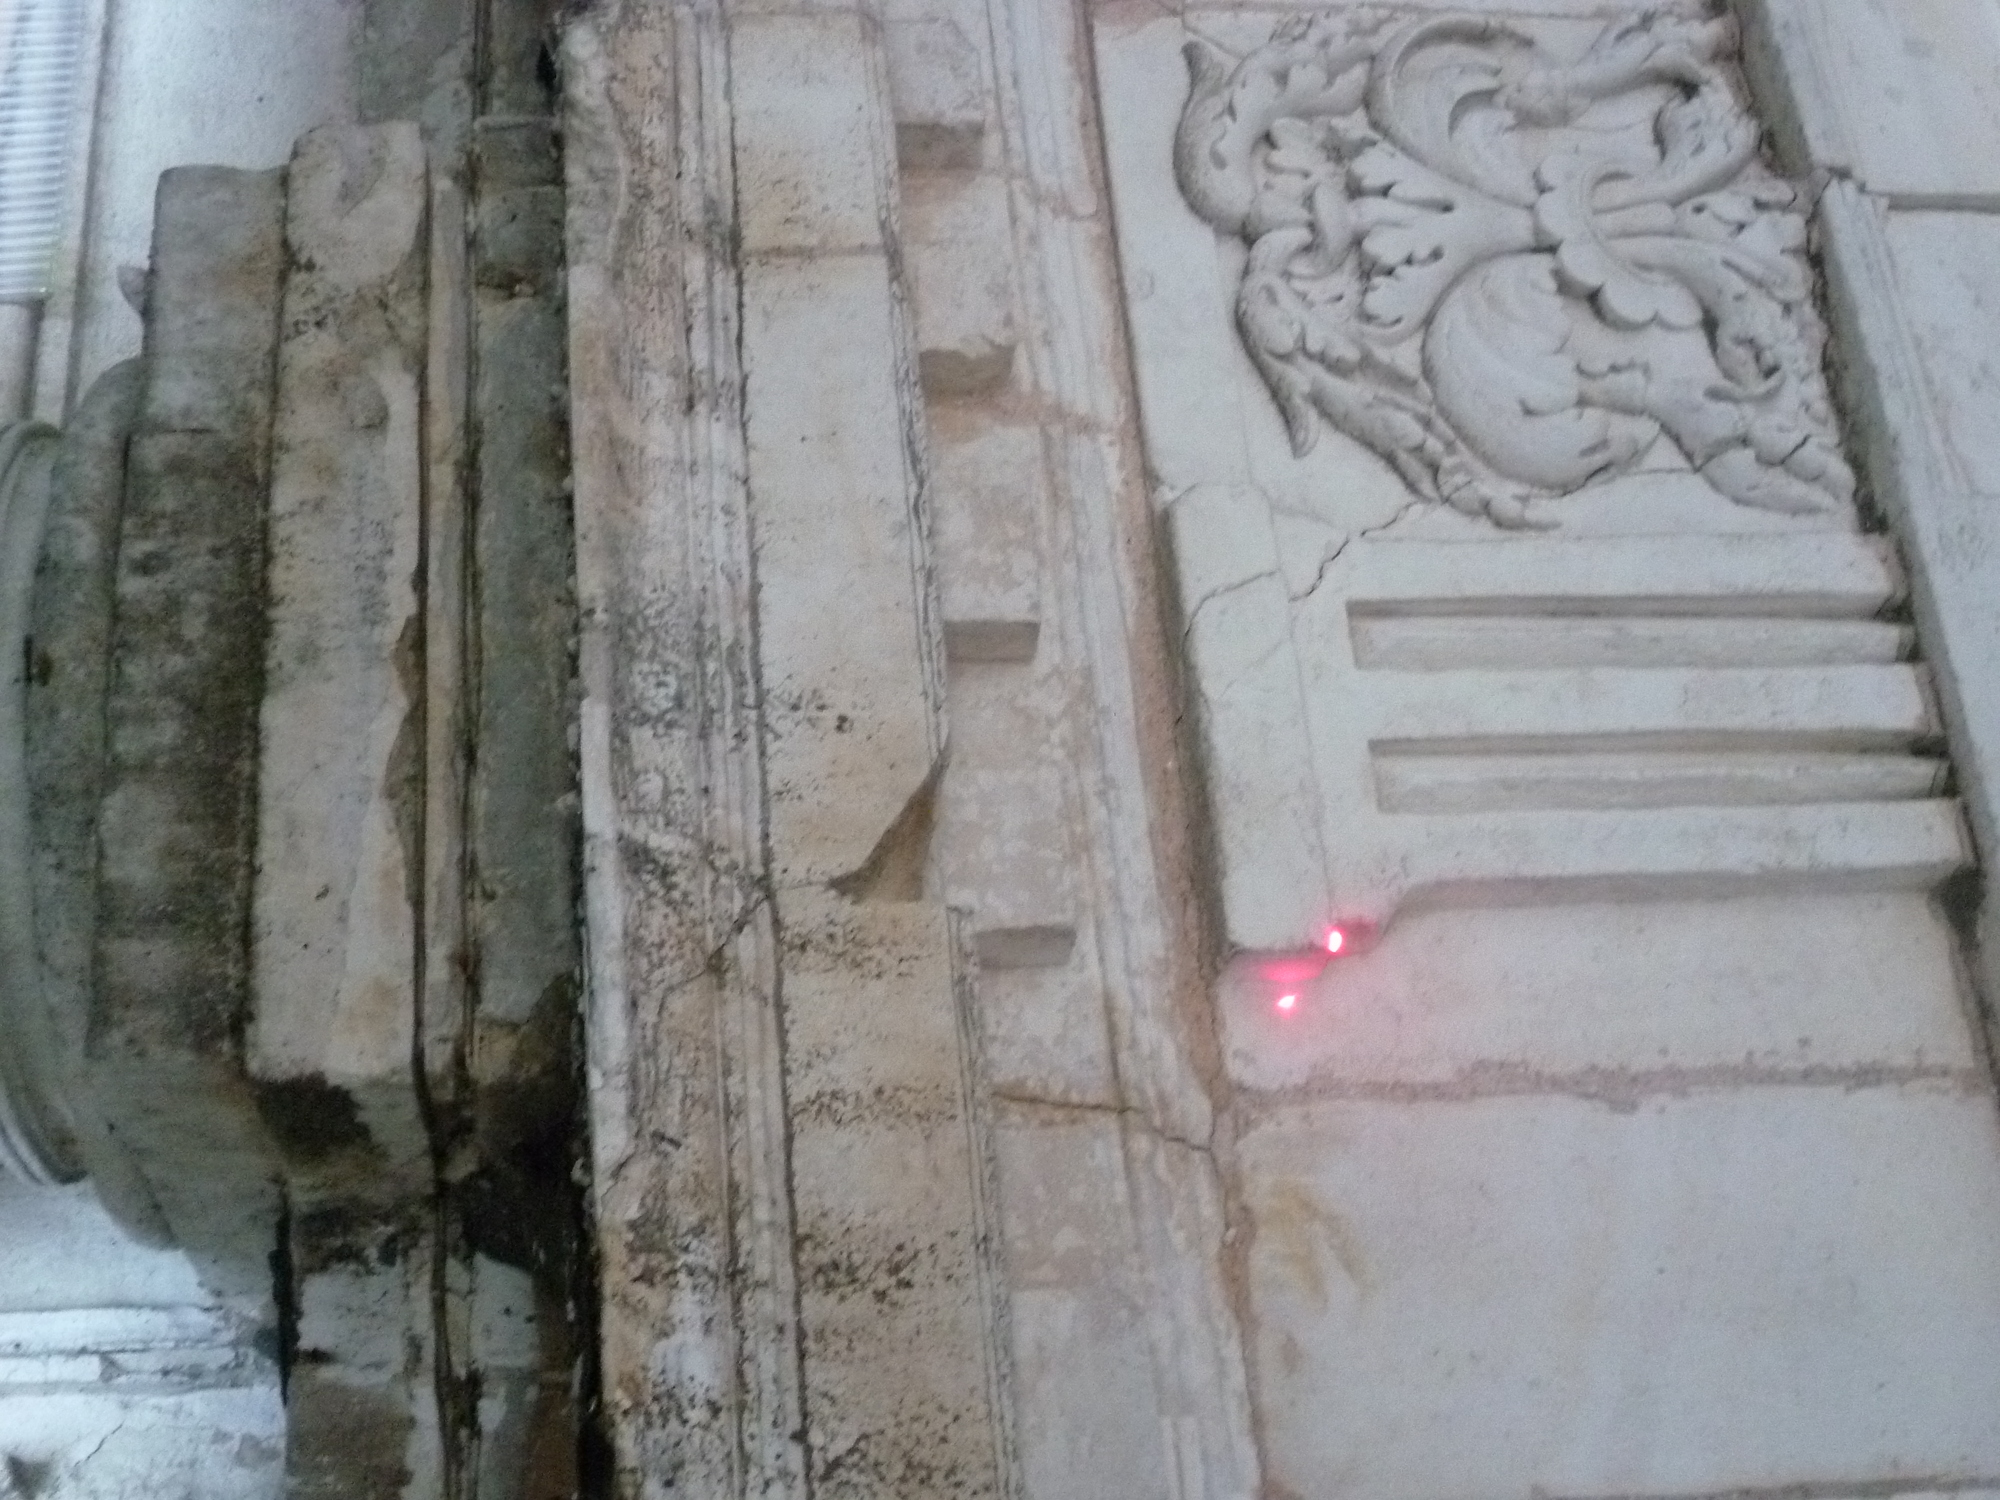
\includegraphics[bb=0 0 2880 2160,trim=0 0 400 300,width=500pt,keepaspectratio=true]{photo538.JPG}
%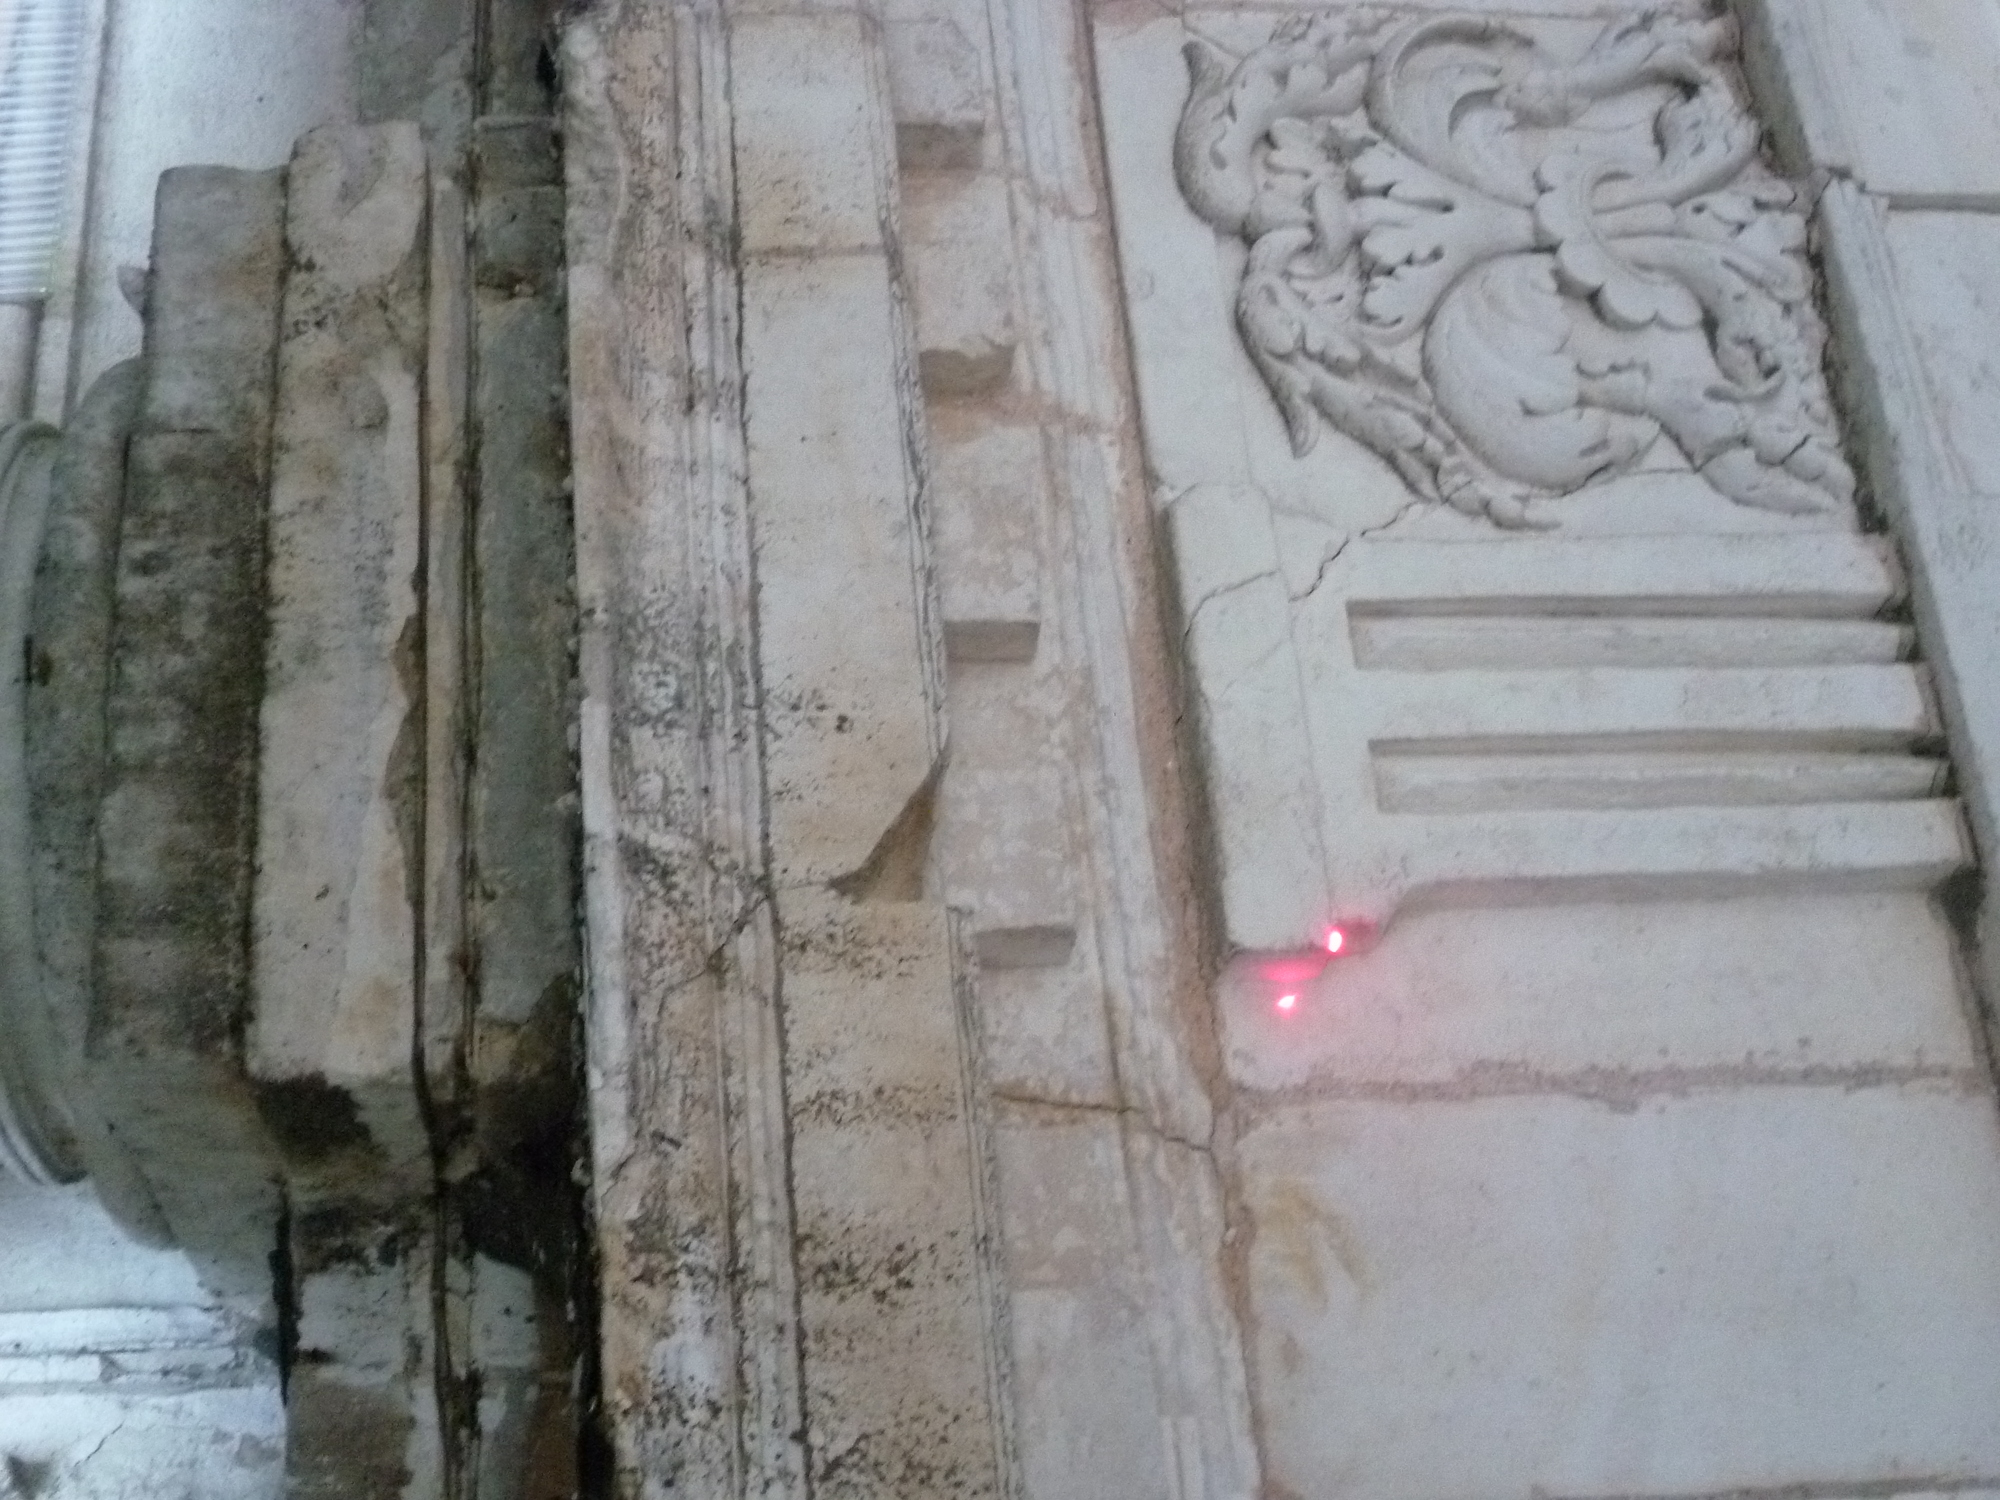
\includegraphics[trim=0 0 100 100,width=300pt,keepaspectratio=true]{photo538.JPG}
%
\includegraphics[bb=0 0 400 300,width=400pt,keepaspectratio=true]{test.jpg}
%
\includegraphics[bb=0 0 400 300,viewport=0 0 400 300,width=400pt,keepaspectratio=true]{test.jpg}
%
\includegraphics[bb=0 0 400 300,trim=0 0 399 299,width=400pt,keepaspectratio=true]{test.jpg}
%\includegraphics[trim=0 0 3000 2000,width=300pt,keepaspectratio=true]{P1020538.JPG}
%\includegraphics[width=100pt]{p1020538.jpg}
%\caption{Point 1009}
%\label{mydessin1}
%\end{figure}

\section{Inclure des graphiques dans un rapport}
\subsection{Le problème}
Nous avons inserer dans notre document une photo.
Quand on compile le document tex, le message d'erreur mentionne l'absence d'un fichier photo.bb.
Ce type de fichier n'est donc pas créé de manière dynamique.
Il est possible de créer ce fichier avec l'utilitaire ebb, mais celui ci donne des bounding box
différentes que l'utilitaire identify

La solution consiste donc à jouer avec les options d'inclusion

\subsection{Les Options}

Nous allons travailler à partir de cette photo qui a été réalisée à l'aide de cette commande :
convert -resize 400x300 logo: test.jpg

\subsubsection{viewport}

L'option viewport fonctionne avec des coordonnées absolues.
Ainsi, {160 120 360 270} correspond à une zone partant du point {160 120}
et allant jusqu'au point {360 270}.
Cela correspond a une image de 200x150.

Sur la figure~\ref{viewport variant et bb constant}, page~\pageref{viewport variant et bb constant},
nous avons, sur les deux premières lignes, un decoupage sans déformation de l'image, 
tandis que, sur la troisième ligne, nous avons un découpage avec déformation de l'image.

% debut d'une premiere figure
\begin{figure}[!h]
  \centering
  %
\includegraphics[width=\textwidth]{mydessin.pdf}
  
\includegraphics[bb=0 0 400 300,height=3cm]{test.jpg}
  \caption{La photo originale}
  \label{Photo originale}
\end{figure}

% debut d'une seconde figure
\begin{figure}[h]
    \centering
    \begin{subfigure}[b]{0.3\textwidth}
        
\includegraphics[viewport=0 0 400 300,bb=0 0 400 300,width=4cm,height=3cm,clip=true]{test.jpg}
        \caption{viewport=0 0 400 300\\bb=0 0 400 300}
        \label{essai_a}
    \end{subfigure}
    ~ %add desired spacing between images, e. g. ~, \quad, \qquad etc.
      %(or a blank line to force the subfigure onto a new line)
    \begin{subfigure}[b]{0.3\textwidth}
        
\includegraphics[viewport=160 120 360 270,bb=0 0 400 300,width=4cm,height=3cm,clip=true]{test.jpg}
        \caption{viewport=160 120 360 270\\bb=0 0 400 300}%+200+150
        \label{essai_b}
    \end{subfigure}
    ~
    \begin{subfigure}[b]{0.3\textwidth}
        
\includegraphics[viewport=160 120 320 240,bb=0 0 400 300,width=4cm,height=3cm,clip=true]{test.jpg}
        \caption{viewport=160 120 320 240\\bb=0 0 400 300}%+160+120
        \label{essai_c}
    \end{subfigure}
    \\
    \begin{subfigure}[b]{0.3\textwidth}
        
\includegraphics[viewport=160 120 280 210,bb=0 0 400 300,width=4cm,height=3cm,clip=true]{test.jpg}
        \caption{viewport=160 120 280 210\\bb=0 0 400 300}%+120+90
        \label{essai_d}
    \end{subfigure}
    ~
    \begin{subfigure}[b]{0.3\textwidth}
        
\includegraphics[viewport=160 120 240 180,bb=0 0 400 300,width=4cm,height=3cm,clip=true]{test.jpg}
        \caption{viewport=160 120 240 180\\bb=0 0 400 300}%+80+60
        \label{essai_e}
    \end{subfigure}
    ~
    \begin{subfigure}[b]{0.3\textwidth}
        
\includegraphics[viewport=160 120 200 150,bb=0 0 400 300,width=4cm,height=3cm,clip=true]{test.jpg}
        \caption{viewport=160 120 200 150\\bb=0 0 400 300}%+40+30
        \label{essai_f}
    \end{subfigure}
    \\
    \begin{subfigure}[b]{0.3\textwidth}
        
\includegraphics[viewport=160 120 240 210,bb=0 0 400 300,width=4cm,height=3cm,clip=true]{test.jpg}
        \caption{viewport=160 120 240 210\\bb=0 0 400 300}%+80+90
        \label{essai_g}
    \end{subfigure}
    ~
    \begin{subfigure}[b]{0.3\textwidth}
        
\includegraphics[viewport=160 120 240 180,bb=0 0 400 300,width=4cm,height=3cm,clip=true]{test.jpg}
        \caption{viewport=160 120 240 180\\bb=0 0 400 300}%+80+60
        \label{essai_h}
    \end{subfigure}
    ~
    \begin{subfigure}[b]{0.3\textwidth}
        
\includegraphics[viewport=160 120 240 150,bb=0 0 400 300,width=4cm,height=3cm,clip=true]{test.jpg}
        \caption{viewport=160 120 240 150\\bb=0 0 400 300}%+80+30
        \label{essai_i}
    \end{subfigure}
    \caption{Les options pour l'insertion d'une image :\\viewport variant et bb constant}%\label{fig-double}
    \label{viewport variant et bb constant}

\end{figure}


% debut d'une troisieme figure
\begin{figure}[h]
    \centering
    \begin{subfigure}[b]{0.3\textwidth}
        
\includegraphics[viewport=0 0 400 300,bb=0 0 400 300,width=4cm,height=3cm,clip=true]{test.jpg}
        \caption{viewport=0 0 400 300\\bb=0 0 400 300}
        \label{essai_a}
    \end{subfigure}
    ~
    \begin{subfigure}[b]{0.3\textwidth}
        
\includegraphics[viewport=0 0 400 300,bb=160 120 400 300,width=4cm,height=3cm,clip=true]{test.jpg}
        \caption{viewport=0 0 400 300\\bb=160 120 400 300}
        \label{essai_2}
    \end{subfigure}
    ~
    \begin{subfigure}[b]{0.3\textwidth}
        
\includegraphics[viewport=0 0 400 300,bb=0 0 0 0,width=4cm,height=3cm,clip=true]{test.jpg}
        \caption{viewport=0 0 400 300\\bb=0 0 0 0}
        \label{essai_3}
    \end{subfigure}
    \caption{Les options pour l'insertion d'une image :\\viewport constant et bb inutile}%\label{fig-double}
    \label{viewport constant et bb inutile}

\end{figure}

\subsubsection{trim}
L'option trim fonctionne avec des coordonnées relatives.
Ainsi, {160 120 40 30} correspond à une zone partant du point {160 120}
et allant jusqu'au point situé à {-40 -30} par rapport au point haut droit.
Si l'image de départ a pour dimension {400 300}, alors effectivement, 
en coordonnées absolues, nous avons {160 120 360 270}.
Cela correspond a une image de 200x150.

Sur la figure~\ref{bb constant et trim variant}, page~\pageref{bb constant et trim variant},
nous avons, sur les deux premières lignes, un decoupage sans déformation de l'image, 
tandis que, sur la troisième ligne, nous avons un découpage avec déformation de l'image.

% debut d'une quatrième figure
\begin{figure}[h]
    \centering
    \begin{subfigure}[b]{0.3\textwidth}
        
\includegraphics[bb=0 0 400 300,trim=0 0 0 0,width=4cm,height=3cm,clip=true]{test.jpg}
        \caption{bb=0 0 400 300\\trim=0 0 0 0}
        \label{essai_4}
    \end{subfigure}
    ~
    \begin{subfigure}[b]{0.3\textwidth}
        
\includegraphics[bb=0 0 400 300,trim=160 120 40 30,width=4cm,height=3cm,clip=true]{test.jpg}
        \caption{bb=0 0 400 300\\trim=160 120 40 30}%
        \label{essai_5}
    \end{subfigure}
    ~
    \begin{subfigure}[b]{0.3\textwidth}
        
\includegraphics[bb=0 0 400 300,trim=160 120 80 60,width=4cm,height=3cm,clip=true]{test.jpg}
        \caption{bb=0 0 400 300\\trim=160 120 80 60}%
        \label{essai_6}
    \end{subfigure}
    \\
    \begin{subfigure}[b]{0.3\textwidth}
        
\includegraphics[bb=0 0 400 300,trim=160 120 120 90,width=4cm,height=3cm,clip=true]{test.jpg}
        \caption{bb=0 0 400 300\\trim=160 120 120 90}%
        %
\includegraphics[viewport=0 0 400 300,bb=0 0 400 300,trim=0 0 0 0,width=4cm,height=3cm,clip=true]{test.jpg}
        %\caption{viewport=0 0 400 300\\bb=0 0 400 300\\trim=0 0 0 0}
        \label{essai_4}
    \end{subfigure}
    ~
    \begin{subfigure}[b]{0.3\textwidth}
        
\includegraphics[bb=0 0 400 300,trim=160 120 160 120,width=4cm,height=3cm,clip=true]{test.jpg}
        \caption{bb=0 0 400 300\\trim=160 120 160 120}%
        %
\includegraphics[viewport=0 0 400 300,bb=0 0 400 300,trim=50 50 60 60,width=4cm,height=3cm,clip=true]{test.jpg}
        %\caption{viewport=0 0 400 300\\bb=0 0 400 300\\trim=50 50 60 60}
        \label{essai_5}
    \end{subfigure}
    ~
    \begin{subfigure}[b]{0.3\textwidth}
        
\includegraphics[bb=0 0 400 300,trim=160 120 200 150,width=4cm,height=3cm,clip=true]{test.jpg}
        \caption{bb=0 0 400 300\\trim=160 120 200 150}%
        %
\includegraphics[viewport=0 0 400 300,bb=0 0 400 300,trim=100 100 110 110,width=4cm,height=3cm,clip=true]{test.jpg}
        %\caption{viewport=0 0 400 300\\bb=0 0 400 300\\trim=100 100 110 110}
        \label{essai_6}
    \end{subfigure}
    \\
    \begin{subfigure}[b]{0.3\textwidth}
        
\includegraphics[bb=0 0 400 300,trim=160 120 160 90,width=4cm,height=3cm,clip=true]{test.jpg}
        \caption{bb=0 0 400 300\\trim=160 120 160 90}%deformation
        %
\includegraphics[viewport=0 0 400 300,bb=0 0 400 300,trim=0 0 0 0,width=4cm,height=3cm,clip=true]{test.jpg}
        %\caption{viewport=0 0 400 300\\bb=0 0 400 300\\trim=0 0 0 0}
        \label{essai_7}
    \end{subfigure}
    ~
    \begin{subfigure}[b]{0.3\textwidth}
        
\includegraphics[bb=0 0 400 300,trim=160 120 160 120,width=4cm,height=3cm,clip=true]{test.jpg}
        \caption{bb=0 0 400 300\\trim=160 120 160 120}
        %
\includegraphics[viewport=0 0 400 300,bb=0 0 400 300,trim=50 50 60 60,width=4cm,height=3cm,clip=true]{test.jpg}
        %\caption{viewport=0 0 400 300\\bb=0 0 400 300\\trim=50 50 60 60}
        \label{essai_8}
    \end{subfigure}
    ~
    \begin{subfigure}[b]{0.3\textwidth}
        
\includegraphics[bb=0 0 400 300,trim=160 120 160 150,width=4cm,height=3cm,clip=true]{test.jpg}
        \caption{bb=0 0 400 300\\trim=160 120 160 150}
        %
\includegraphics[viewport=0 0 400 300,bb=0 0 400 300,trim=100 100 110 110,width=4cm,height=3cm,clip=true]{test.jpg}
        %\caption{viewport=0 0 400 300\\bb=0 0 400 300\\trim=100 100 110 110}
        \label{essai_9}
    \end{subfigure}
    \caption{Les options pour l'insertion d'une image :\\bb constant et trim variant}%\label{fig-double}
    \label{bb constant et trim variant}

\end{figure}


% debut d'une cinquieme figure
\begin{figure}[h]
    \centering
    \begin{subfigure}[b]{0.3\textwidth}
        
\includegraphics[bb=0 0 400 300,trim=0 0 0 0,width=4cm,height=3cm,clip=true]{test.jpg}
        \caption{bb=0 0 400 300\\trim=0 0 0 0}
        \label{essai_a}
    \end{subfigure}
    ~
    \begin{subfigure}[b]{0.3\textwidth}
        
\includegraphics[bb=160 120 560 420,trim=0 0 0 0,width=4cm,height=3cm,clip=true]{test.jpg}
        \caption{bb=160 120 560 420\\trim=0 0 0 0}
        \label{essai_2}
    \end{subfigure}
    ~
    \begin{subfigure}[b]{0.3\textwidth}
        
\includegraphics[bb=160 120 400 300,trim=0 0 0 0,width=4cm,height=3cm,clip=true]{test.jpg}
        \caption{bb=160 120 400 300\\trim=0 0 0 0}
        \label{essai_3}
    \end{subfigure}
    \caption{Les options pour l'insertion d'une image :\\bb inutile et trim constant}%\label{fig-double}
    \label{bb inutile et trim constant}

\end{figure}


% debut d'une troisieme figure
\begin{figure}[!h]
\centering
%
\includegraphics[width=\textwidth]{mydessin.pdf}

\includegraphics[width=300pt]{mydessin.pdf}
\caption{Ceci est encore mydessin.pdf}
\label{mydessin3}
\end{figure}

% debut d'une quatrieme figure
\begin{figure}[!h]
\centering
%
\includegraphics[width=\textwidth]{mydessin.pdf}
\includegraphics[width=400pt]{mydessin.pdf}
\caption{Ceci est encore et toujours mydessin.pdf}
\label{mydessin4}
\end{figure}

% reference a une figure
Sur la figure~\ref{mydessin1}, page~\pageref{mydessin1}, nous avons mis une largeur de 100 pt.

Sur la figure~\ref{mydessin2}, page~\pageref{mydessin2}, nous avons mis une largeur de 200 pt.

Sur la figure~\ref{mydessin3}, page~\pageref{mydessin3}, nous avons mis une largeur de 300 pt.

Sur la figure~\ref{mydessin4}, page~\pageref{mydessin4}, nous avons mis une largeur de 400 pt.

% liste des figures
\listoffigures

\end{document}
